\documentclass[11pt,letterpaper,titlepage]{article}

\usepackage[pdftex]{graphicx}
\usepackage{multicol}
\usepackage{subfig}
\usepackage{wrapfig}

\begin{document}

%%%%%%%% TITLE PAGE %%%%%%%%%%%%%%%%%%%%%%%%%%%%%%%%%%%%%%%%%%%%%%%%%%%%%%%%%%%%%%%%%%%%%%%%%%%%%%%%%%%%%%%%%%%%%%%%%%%%%%%%%%%%%%%

\title{ECE 2220 Final Design Project}
\author{Burke Libbey \\ John Ermitanio \\ Crystal Kotlar}
\date{December 3, 2007}
\maketitle

%%%%%%%% TABLE OF CONTENTS %%%%%%%%%%%%%%%%%%%%%%%%%%%%%%%%%%%%%%%%%%%%%%%%%%%%%%%%%%%%%%%%%%%%%%%%%%%%%%%%%%%%%%%%%%%%%%%%%%%%%%%%%

\tableofcontents
\listoffigures
\newpage

%%%%%%%% CONTENT %%%%%%%%%%%%%%%%%%%%%%%%%%%%%%%%%%%%%%%%%%%%%%%%%%%%%%%%%%%%%%%%%%%%%%%%%%%%%%%%%%%%%%%%%%%%%%%%%%%%%%%%%%%%%%%%%%%

%%%%%%%%%%%%%%%%%%%%%%%%%%%%%%%%%%%%%% INTRODUCTION %%%%%%%%%%%%%%%%%%%%%%%%%%%%%%%%%%%%%%
\section{Introduction}

Aircraft often use Non-Directional Beacons (NDBs) to determine their position. These beacons transmit a morse code callsign, the strength of which is used to calculate the distance from the beacon to the aircraft. It is very important that these beacons continue to function properly, so an autonomous beacon monitoring system is necessary.

Using an Altera FPGA and Quartus II software, our team designed a prototype system to autonomously monitor the output transmission of a selected aircraft navigation beacon.


%%%%%%%%%%%%%%%%%%%%%%%%%%%%%%%%%%%%%% DESIGN AND IMPLEMENTATION %%%%%%%%%%%%%%%%%%%%%%%%%%%%%%%%%%%%%%
\section{Design and Implementation}
%%%%%%%%%%%%%%%%%%% OVERVIEW %%%%%%%%%%%%%%%%%%%
\subsection{Overview}

Two distinct two-character sequences are stored in a series of shift registers. A keypad is used to select one of the two sequences, which is then sequentially unloaded into the comparator circuit, which compares the stored sequence against the incoming morse code input from a pushbutton. If the two signals differ on a negative clock edge, an error condition is raised and the system waits for a reset. If the signal matches successfully, a green LED is lit and the system waits for keypad input to begin listening for another sequence.

\begin{figure}[!htb]
	\begin{center}
		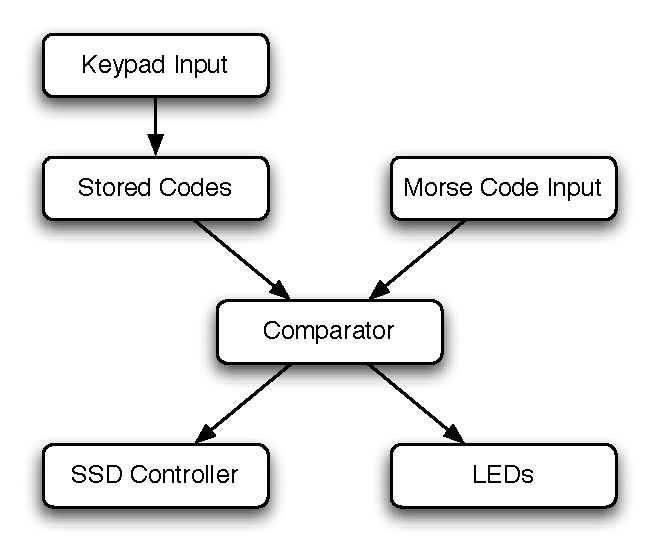
\includegraphics[width=2.5in]{graphics/highlevelarchitecture.pdf}
		\caption{Overview of Project Architecture}
		\label{fig:Overview}
	\end{center}
\end{figure}

%%%%%%%%%%%%%%%%%%% INPUT %%%%%%%%%%%%%%%%%%%
\subsection{Input}
\subsubsection{Keypad}
The `\texttt{0}' (AB) and `\texttt{1}' (CD) buttons on the project board keypad are used to select one of two stored sequences. These sequences are stored using a modified morse code, defined by the following rules:
\begin{itemize}
\small
\item Dashes convert to three consecutive `\texttt{1}'s.
\item Dots convert to a single `\texttt{1}'.
\item A single `\texttt{0}' is inserted between each dot or dash.
\item Three consecutive `\texttt{0}'s are inserted between letters.
\item Seven `\texttt{0}'s are inserted after each word.
\end{itemize}

\begin{figure}[!htb]
	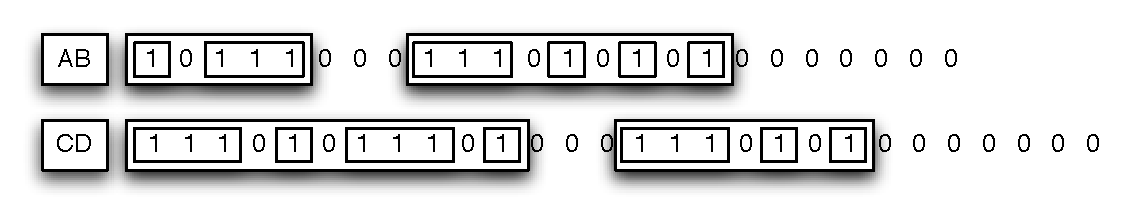
\includegraphics[width=5in]{graphics/morseencoded.pdf}
	\caption{Selected encoded sequences}
	\label{fig:MorseEncoded}
\end{figure}

When one of the defined buttons on the keypad is pressed, both shift registers begin simultaneously unloading into the \textit{selector} (\S\ref{ssS:selector}) on the positive clock edge. 
\subsubsection{Pushbutton}\label{ssS:pushbutton}
A pushbutton is used as the morse code input (analogous to the transmitted signal from the beacon), for comparison against the selected stored input. This input is passed directly to the \textit{comparator} (\S\ref{ssS:comparator}).

%%%%%%%%%%%%%%%%%%% LOGIC %%%%%%%%%%%%%%%%%%%
\subsection{Logic}
\subsubsection{Selector}\label{ssS:selector}


\begin{figure}[!htb]
	\begin{center}
		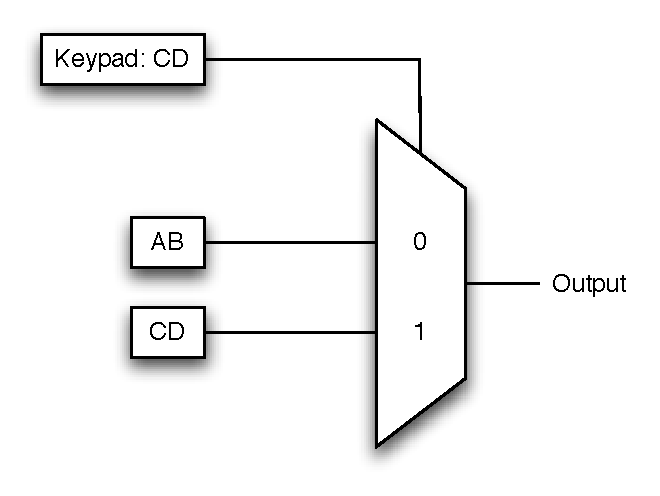
\includegraphics[width=2.5in]{graphics/selector.pdf}
		\caption{Selector}
		\label{fig:Selector}
	\end{center}
\end{figure}


When the `\texttt{1}' key is pressed, a D flip-flop is set to High. It is reset to Low when `\texttt{0}' is pressed. This flip-flop serves as the select input for a multiplexer fed both of the now-unloading shift registers. The net effect is to output `AB' or `CD' from the multiplexer, depending on whether `\texttt{0}' or `\texttt{1}' is pressed.



\subsubsection{Comparator}\label{ssS:comparator}


\begin{figure}[!htb]
	\begin{center}
		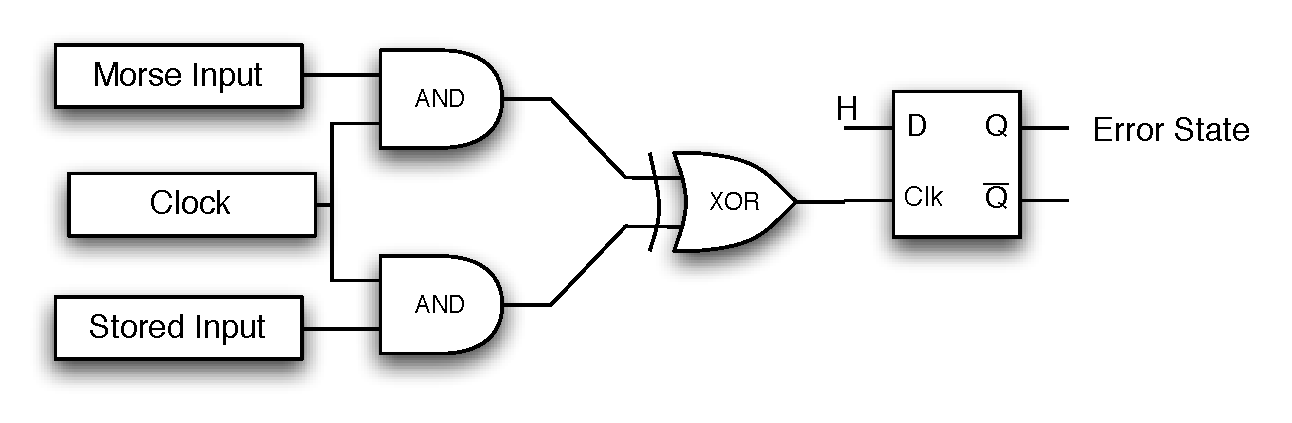
\includegraphics[width=5in]{graphics/comparator.pdf}
		\caption{Comparator}
		\label{fig:Comparator}
	\end{center}
\end{figure}


The comparator is used to compare the selected stored input and the incoming morse signal. Each of the inputs is \texttt{AND}ed with the 1Hz clock and fed to an \texttt{XNOR} gate. This gate will output High when there is a difference in the incoming data. This output is passed to a D flip-flop such that the \texttt{Q} output of the flip-flop is initially Low, then goes permanently High the first time the Data line (\texttt{XNOR} output) goes High. The system then waits for a manual reset, as an error has been encountered.

\subsubsection{Zero-overflow Detection}\label{ssS:ZOD}

\begin{figure}
	\begin{center}
		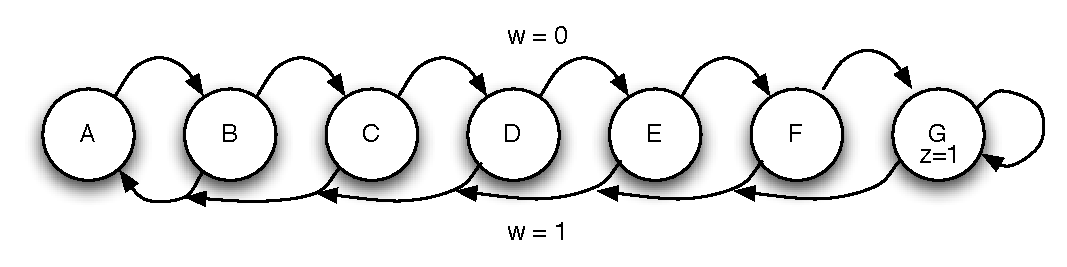
\includegraphics[width=4.5in]{graphics/fsm.pdf}
		\caption{State diagram for zero detection}
		\label{fig:FSM}
	\end{center}
\end{figure}

This subsystem runs parallel to the comparator. When a sequence of seven sequential zeroes is encountered and no errors have been raised, the output is verified. If a sequence of 8 or more zeroes is encountered, a timeout has occurred and an error is raised. The zero-overflow detection circuit was implemented with a finite state machine.

%%%%%%%%%%%%%%%%%%% OUTPUT %%%%%%%%%%%%%%%%%%%
\subsection{Output}
\subsubsection{LEDs}\label{ssS:leds}

Three LEDs are used:
\begin{itemize}
	\item \textbf{Green}: Indicates that the previous sequence was correct.
	\item \textbf{Yellow}: Indicates that a sequence is currently in transmission.
	\item \textbf{Red}: Indicates that an error occurred and the system must be reset.
\end{itemize}


\subsubsection{Seven Segment Displays}\label{ssS:ssd}
The Seven-Segment Displays on the project board are used to display the sequence currently being transmitted, the sequence successfully matched, or `EE' in case of an error condition. \textit{(Fig. \ref{fig:SSD})}

\begin{figure}[!htb]
  \centering
  \subfloat[AB]{\label{fig:AB}
    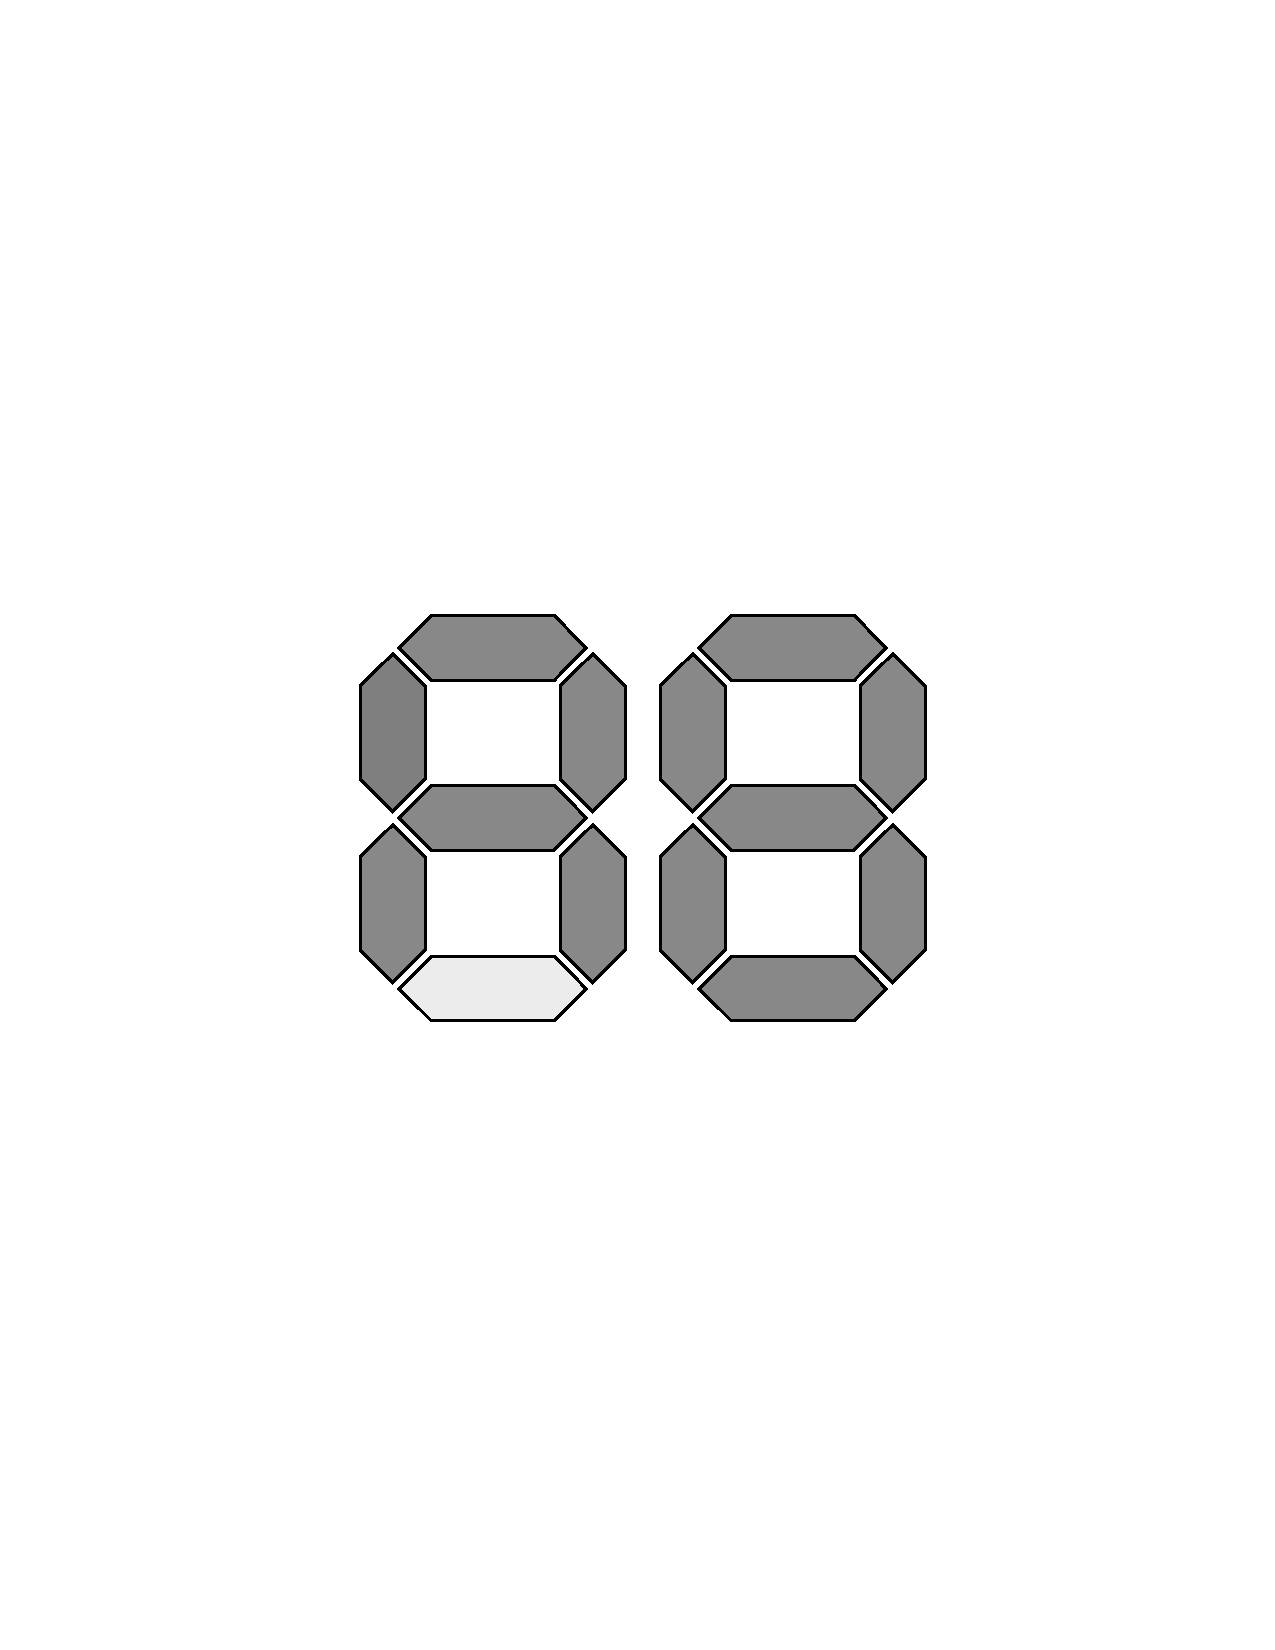
\includegraphics[width=1in]{graphics/AB.pdf}}
  \quad
  \subfloat[CD]{\label{fig:CD}
    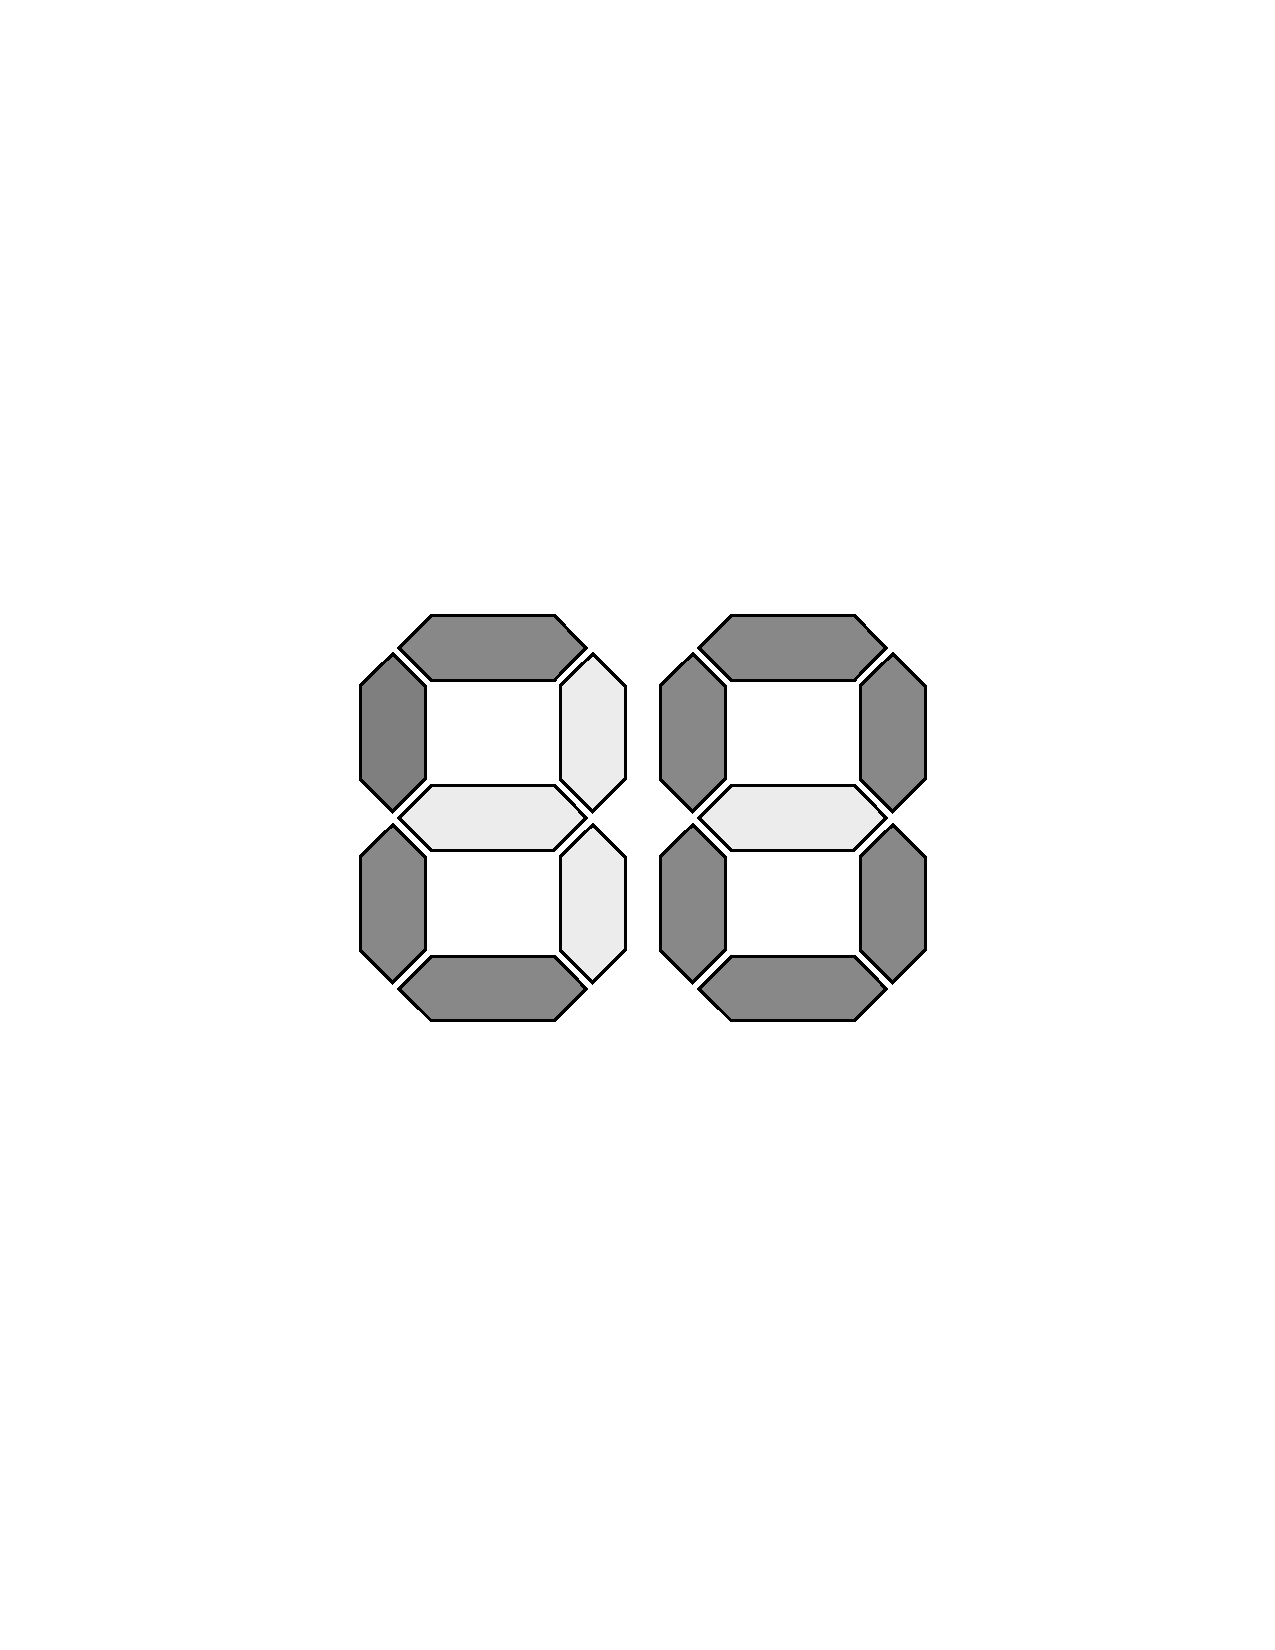
\includegraphics[width=1in]{graphics/CD.pdf}}
  \quad
  \subfloat[EE]{\label{fig:EE}
    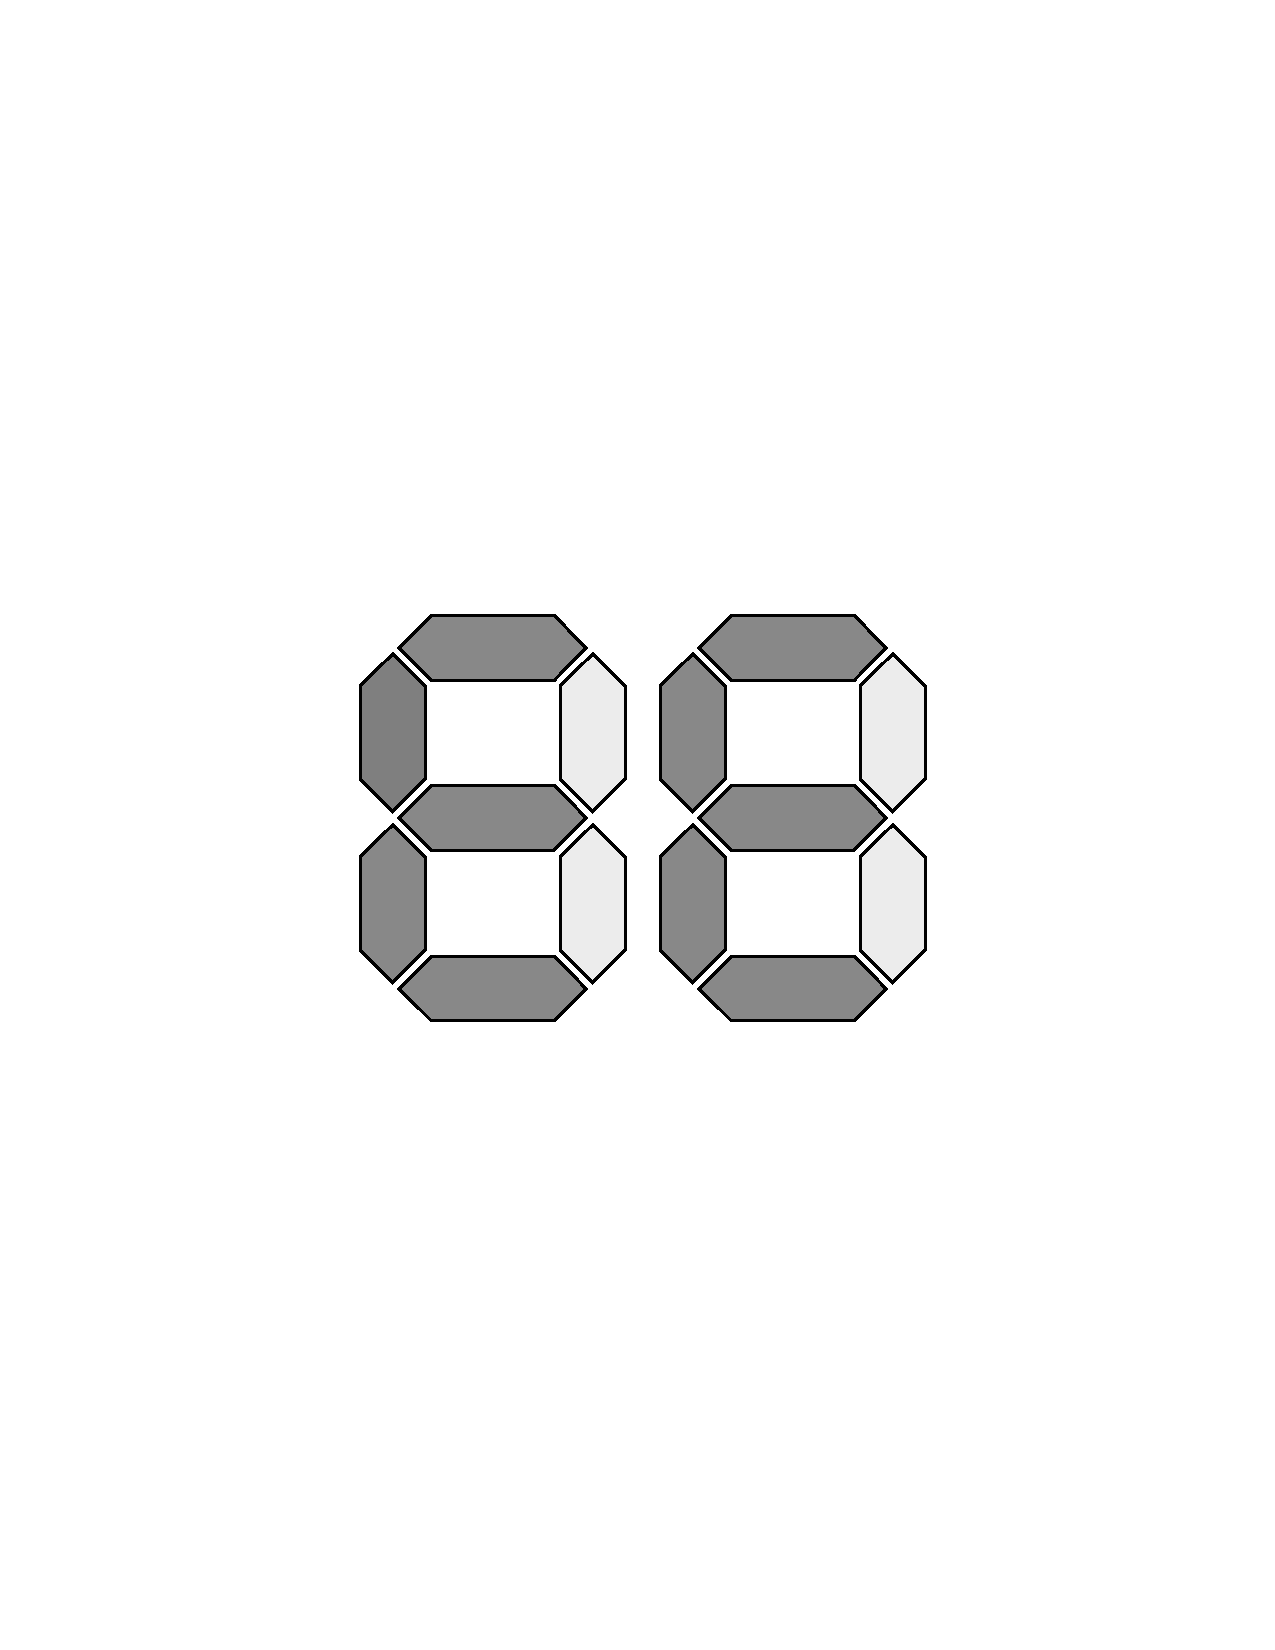
\includegraphics[width=1in]{graphics/EE.pdf}}
  \caption{Possible SSD output values}
  \label{fig:SSD}
\end{figure}



%%%%%%%%%%%%%%%%%%%%%%%%%%%%%%%%%%%%%% UNIMPLEMENTED IDEAS %%%%%%%%%%%%%%%%%%%%%%%%%%%%%%%%%%%%%%
\section{Unimplemented Ideas}
\subsection{BCD Zero Counter}

\textbf{The idea:} To use a BCD counter to detect 7 and 8 sequential zeroes on the morse code input line (\S\ref{ssS:ZOD}). Given the outputs $\{A, B, C, D\}$, a sequence of seven zeroes is given by $ABC$, and eight by $D$.

\noindent\textbf{Why it wasn't implemented:} The project requirements specified that we must use at least one finite state machine. We felt we had found better solutions for every opportunity, and this was the one we felt least strongly about, hence, it was implemented with a FSM rather than a BCD.


%%%%%%%%%%%%%%%%%%%%%%%%%%%%%%%%%%%%%% PROBLEMS WE ENCOUNTERED %%%%%%%%%%%%%%%%%%%%%%%%%%%%%%%%%%%%%%
\section{Problems we Encountered}
\subsection{Manual Input}
The first significant problem we had related to the timing of the shift registers that stored the encoded morse code. Originally, the shift register enable was tied to a switch ($S_{6a}$). The switch was initially low, then set high when the registers should start unloading. This meant that to start unloading the shift register at the appropriate time, one would have to press the keypad button and flip a switch at the same time. This problem was corrected by passing our two keypad inputs each into a D flip-flop to store whether they had been pressed yet. The \texttt{OR} of these two flip-flops was used in place of the switch we had used initially.

\subsection{Quartus Quirks}
The single most common error we encountered was in copying and pasting parts of our schematic between \textit{Block Diagram Files}. Lines would often accidentally be crossed in very inappropriate places. This was often caught with a compile-time error, but on a couple occasions, we had to carefully scan our circuit for unintentionally crossed lines.

\subsection{D Flip-flop Initial Condition}
We ran into trouble several times trying to use D flip-flops as latches. Our intention was to have $Q$ stay low until the first high was encountered on $D$, then to have $Q$ stay permanently high. We tried several configurations, each with very limited or no success. In the end, we succeeded by feeding the inverted output line back to the $PRN$. 



%%%%%%%%%%%%%%%%%%%%%%%%%%%%%%%%%%%%%% SIMULATIONS %%%%%%%%%%%%%%%%%%%%%%%%%%%%%%%%%%%%%%
\section{Simulations}

\begin{figure}[!htb]
	\begin{center}
		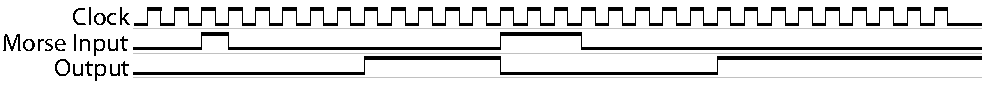
\includegraphics[width=5in]{graphics/sim/fsmsimulation.pdf}
		\caption{Simulation of Zero-detection Finite State Machine}
		\label{fig:FSMSim}
	\end{center}
\end{figure}


\begin{figure}[!htb]
	\begin{center}
		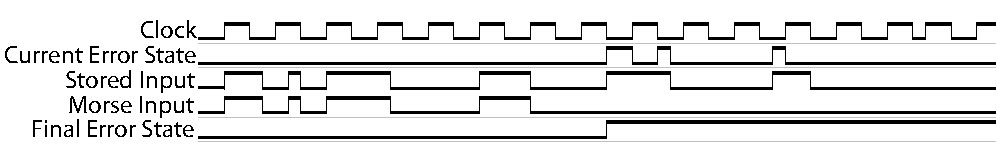
\includegraphics[width=5in]{graphics/sim/comparatorsimulation.pdf}
		\caption{Simulation of Comparator}
		\label{fig:CompSim}
	\end{center}
\end{figure}


%%%%%%%%%%%%%%%%%%%%%%%%%%%%%%%%%%%%%% CONCLUSION %%%%%%%%%%%%%%%%%%%%%%%%%%%%%%%%%%%%%%
\section{Conclusion}
This project was an exercise in debugging. Most of our problems arose from not testing component circuits thoroughly before combining parts. Much effort could have been saved if we had done more testing along the way. In future projects, we would run tests much more frequently.

Additionally, we discovered that partitioning a poorly-understood project into poorly-understood component tasks does not work well. In the future, we would spend more time as a group trying to fully understand the scope of the project.
\newpage
\begin{figure}
	\vspace{-0.7in}

	\begin{center}
		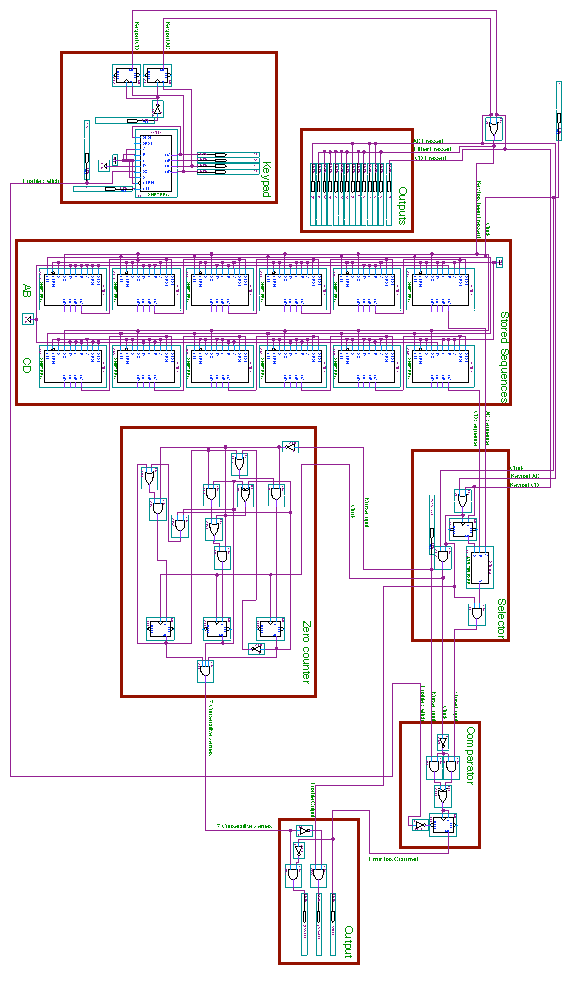
\includegraphics[width=4.6in]{graphics/schematic.pdf}
		\caption{Full schematic of final circuit}
		\label{fig:schematic}
	\end{center}
\end{figure}

\end{document}

